\pdfminorversion=4
\documentclass[english]{beamer}
\usepackage{beamerthemesplit}
\usepackage[english]{babel}
\usepackage{graphicx}
\usepackage{fancyvrb}
\usepackage{wrapfig}
\usepackage{xcolor}
\usepackage{fontspec}
\fontspec{Droid Sans}
\fontspec{DejaVu Sans Mono}
\setmainfont[Scale = 0.9]{Droid Sans}
\setsansfont[Scale = 0.9]{Droid Sans}
\setmonofont[Scale = 0.8]{DejaVu Sans Mono}
\newfontfamily\frametitlefont{Droid Sans}

\usetheme[alternativetitlepage=true,titleline=true]{Torino}
\usecolortheme{nouvelle}
\title{\frametitlefont{Le logiciel libre et le Web 2.0}}
\subtitle{{\small Deux mondes intimement liés}}
\author{Jérémie Laval \and Rémy Hubscher}
\date{24 novembre 2011}

\hypersetup{
  pdftitle={Le logiciel libre et le Web 2.0},
  pdfauthor={Jérémie Laval et Rémy Hubscher},
  unicode=true,
  pdfsubject={Le logiciel libre et le Web 2.0}
}

\newenvironment{litemize}
{\begin{itemize}
  \setlength{\itemsep}{1.5em}
  \setlength{\parskip}{0pt}
  \setlength{\parsep}{0pt}}
{\end{itemize}}

\newenvironment{llitemize}
{\begin{itemize}
  \setlength{\itemsep}{0.35em}
  \setlength{\parskip}{0pt}
  \setlength{\parsep}{0pt}}
{\end{itemize}}

\begin{document}

% Infos page
\frame[t,plain]{\titlepage}

% Plan
\begin{frame}[t,plain]{\frametitlefont{Plan}}
  \tableofcontents
\end{frame}

\section{Le Logiciel Libre}
\label{sec:ll}

\subsection{Comparaison}
\label{sec:ll-comparaison}

\begin{frame}[t]{\frametitlefont{La recette de cuisine}}
  \vspace{-2em}
  \center{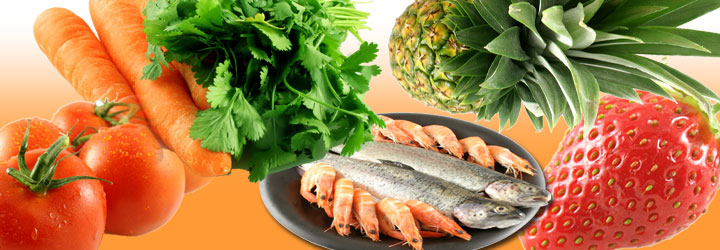
\includegraphics[width=0.75\textwidth]{recette.png}}
  \newline
  \vspace{-.5em}
  \begin{enumerate}
  \item <2-> Pas de restriction d'utilisation.
  \item <3-> Instructions présentes.
  \item <4-> Chacun sa recette.
  \item <5-> Partage.
  \end{enumerate}

  \begin{center}
      \uncover<6->{\Large Normal non ?}
  \end{center}
\end{frame}

\begin{frame}[t]{\frametitlefont{Le cas d'un logiciel}}
  \vspace{-2.5em}
  \begin{center}
    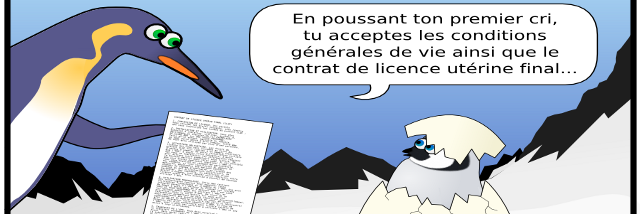
\includegraphics[height=3.5cm]{eula.png}
  \end{center}
  \vspace{-1em}
  \begin{enumerate}
  \item <2-> Contrats, EULA, DRM $ \Rightarrow $ restrictions.
  \item <3-> Exécutable opaque $ \Rightarrow $ pas de code source.
  \item <4-> Modification = contrefaçon $ \Rightarrow $ peine de prison.
  \item <5-> Partager = pirate $ \Rightarrow $ conséquences juridiques.
  \end{enumerate}

  \begin{center}
      \uncover<6->{\Large Alors que c'est aussi une recette de cuisine}
  \end{center}
\end{frame}

\subsection{Une philosophie}

\begin{frame}[t]{\frametitlefont{Une philosophie}}
  \vspace{-2em}
  \begin{center}
    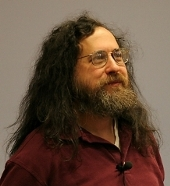
\includegraphics[height=3cm]{stallman.png}
  \end{center}

  4 libertés fondamentales :
  \vspace{1em}
  \begin{enumerate}
  \item <2-> La liberté d'exécuter le programme.
  \item <3-> La liberté d'étudier le fonctionnement du programme.
  \item <4-> La liberté de redistribuer des copies.
  \item <5-> La liberté d'améliorer le programme et de publier ces améliorations.
  \end{enumerate}
  \vfill
\end{frame}

\subsection{Des licences}

\begin{frame}
  \frametitle{Des licences}
  \vspace{-2em}
  \begin{center}
    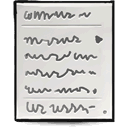
\includegraphics[scale=0.6]{licence.png}
  \end{center}
  \vspace{-1em}
  \begin{itemize}
  \item <2-> Apporter une valeur juridique (copyleft)
  \item <3-> Plusieurs existantes : interprétation différente de liberté
    \begin{itemize}
    \item <4-> GPL (\textit{General Public License}) - FSF
    \item <5-> BSD - Université Berkeley
    \item <6-> MIT - Massachusetts Institute of Technology
    \end{itemize}
  \end{itemize}

\end{frame}

\subsection{Des organisations}

\begin{frame}
  \frametitle{Des organisations}
  \vspace{-.5em}
  \begin{center}
  \visible<2->{\center{
\includegraphics[width=0.70\textwidth]{fsf.png}}}
  \newline
  \visible<3->{\center{
\includegraphics[height=1.8cm]{fsfe.png}}}
  \newline
  \visible<4->{\center{
\includegraphics[height=2.8cm]{april.png}}}
  \end{center}
\end{frame}

\subsection{Avantages pratiques}
\begin{frame}
  \frametitle{Pour le développeur / l'entreprise}
  \vspace{-2em}
  \begin{center}
    
\includegraphics[scale=0.2]{boss.png}
  \end{center}
  \vspace{-1em}
  \begin{itemize}
  \item <2-> Récupérer le savoir existant
  \item <3-> Réutiliser des briques libres
  \item <4-> Code revu, corrigé et amélioré par le monde entier
  \item <5-> Publicité
  \end{itemize}
\end{frame}

\begin{frame}
  \frametitle{Pour l'utilisateur / le client}
  \vspace{-2em}
  \begin{center}
    
\includegraphics[scale=0.2]{catbert.png}
  \end{center}
  \vspace{-1em}
  \begin{itemize}
  \item <2-> Liberté d'utilisation
  \item <3-> Indépendance technologique
  \item <4-> Liberté de concurrence
  \item <5-> Pérénité
  \end{itemize}
\end{frame}

\section{Logiciel Libre et Internet}
\begin{frame}[t]
  \frametitle{Firefox}
  \begin{center}
    
\includegraphics[scale=0.25]{firefox.png} \\
    \vspace{10px}
    {\LARGE \emph{26\%} de part de marché} \\
    Source : StatCounter (novembre 2011)
  \end{center}
\end{frame}

\begin{frame}[t]
  \frametitle{Apache}
  \begin{center}
    
\includegraphics[scale=1.3]{apache.png} \\
    \vspace{10px}
    {\LARGE \emph{65\%} des sites web les plus visités} \\
    Source : Netcraft (novembre 2011)
  \end{center}
\end{frame}

% A faire
% ARPANET -> projet d'université -> bouillon de culture à logiciel libre
% Scratch an itch -> développment logiciel -> mis en logiciel libre
% Infrastructure d'internet repose sur des logiciels libres (mail, dns, ftp, newsgroup)
% Le monde des protocoles et des formats s'en inspirent
% Le libre est un environnement de travail ultra-distribué, Internet relie les développeurs

\end{document}
